\chapter{Lecture two: Classes}
\section{Problem-Domain analysis}
\begin{center}
    Principle: \textit{Model the real world as future users will see it}
\end{center}
\subsection{Results}
The first part of the results is a class diagram. This is essentially what characterises the problem domain. Some structure relations are explained in these types of diagrams.

A behavioural pattern for each class, this describes the behaviour of a class, fields, and functions.

\begin{figure}[H]
    \centering
    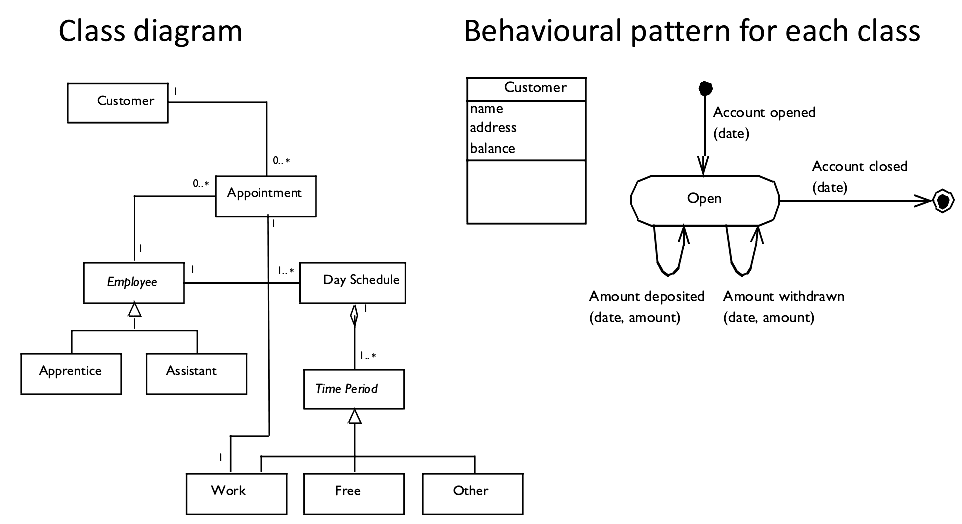
\includegraphics[width=0.75\textwidth]{figures/classdiagandbehaviouralpattern.png}
\end{figure}
\subsection{Key concepts}

\subsubsection{Problem domain}
The \textbf{problem domain} is the part of a context that is administrated, monitored, or controlled by a system. Recall that the \textbf{user} and the \textbf{system} resides in the \textbf{application domain}.

\subsubsection{The model}
The \textbf{model} is a description of classes, objects, structures, and behaviour in a problem domain. This provides an updated representation of the state in the problem domain.

In \textbf{analysis}, we describe the problem domain by an object-oriented model. In \textbf{design}, we adapt this model to become the model component of the system.

\subsection{Summary}
\begin{figure}[H]
    \centering
    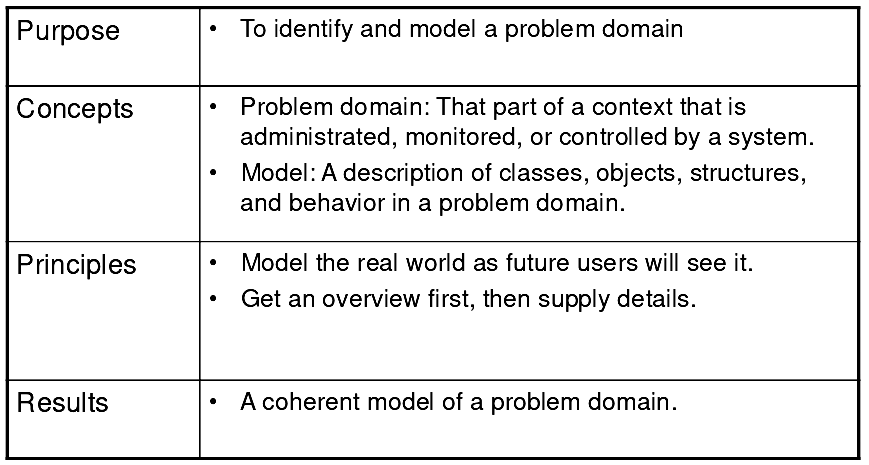
\includegraphics[width=0.75\textwidth]{figures/problemdomainanalysissummary.png}
\end{figure}
\section{The classes activity}
\subsection{Result}
An \textbf{event table}. This shows major classes and events in the problem domain. This is the starting-point for the following activity.

\begin{table}[h]
\centering
\begin{tabular}{l|l|l|l|l|l|l|l|}
\cline{2-8}
 & reserved & cancel & treated & employed & resigned & graduated & agreed \\ \hline
\multicolumn{1}{|l|}{Customer} & \checkmark & \checkmark & \checkmark &  &  &  &  \\ \hline
\multicolumn{1}{|l|}{Assistant} & \checkmark & \checkmark &  & \checkmark & \checkmark &  & \checkmark \\ \hline
\multicolumn{1}{|l|}{Apprentice} &  &  &  & \checkmark & \checkmark & \checkmark & \checkmark \\ \hline
\multicolumn{1}{|l|}{Appointment} & \checkmark & \checkmark & \checkmark &  &  &  &  \\ \hline
\multicolumn{1}{|l|}{Plan} & \checkmark &  &  &  &  &  & \checkmark \\ \hline
\end{tabular}
\caption{Event table for hair salon}
\end{table}

Shows major classes and events in the problem domain. The classes are often listed horizontally, but depends on number of each.

\subsection{Classifying objects and events in the problem domain}
We try to distil the messy real world of classes and objects and events by abstracting and classifying these. 

\subsection{Key concepts}

\subsubsection{Object and class}
An \textbf{object} is an entity with; \textbf{identity, state, and behaviour}. 

\begin{itemize}
    \item[] identity: \texttt{myChair}
    \item[] state: by dining table, free
    \item[] behaviour: bought moved to, ..., sat down on, got up from, ...., moved to, ..., sold
\end{itemize}

\noindent Two kinds of objects: 
\textbf{Analysis objects} describes phenomena outside the system, such as people and things, which are typically independent. although we cannot always command them, we must register the events they perform or experience. \textbf{Design objects} describe phenomena within the system that we can control. We describe their behaviour as operations for the computer to carry out.

\bigskip
\noindent A \textbf{class} is a description of a collection of objects sharing; \textbf{structure, behavioural pattern, and attributes}

\begin{itemize}
    \item[] structure: has an owner
    \item[] attributes: position, vacant
    \item[] behavioural pattern: \texttt{buy + \{move + | sit down on + get up from\}* + sell}
\end{itemize}

\subsubsection{Event}
An event is \textbf{an instantaneous incident involving one or more objects.} Atomic, meaning that they should not be further divisible (if so, use those subevents instead), common to several objects, and have a unique name. At IKEA this could be \texttt{payment\_completed}, when payment and maybe receipt-printing for the cart has been completed.

\subsection{Classes: Activities}
Find candidates for both classes and events, and evaluate these and select systematically. This will result in an event table.

Common techniques for generating candidate lists, e.g. brainstorming, could be to make a list of all potentially relevant classes and events. You should consider many sources; your own perception of the problem domain, existing descriptions (rich pictures, the system definition, etc.), collaboration with prospective users.

Naming must be \textbf{simple} and \textbf{readable} and should originate in the problem domain.

\noindent Classes should be found by looking for nouns, eliminate nouns that reflect administration objects and devices. Make sure to only describe a single instance (object).

\noindent Events should be found by looking for verbs, eliminate verbs related to the way users carry out their job - those related to the application domain. Make sure to only describe a single event - the concept of an \textit{atomic} event.

\subsection{FACTOR example; hair salon}
\begin{itemize}
    \item[] \textbf{Functionality: } Support for work planning and appointments
    \item[] \textbf{Application domain: } Managing customers, their treatments, and appointments, and planning employees' work schedules
    \item[] \textbf{Conditions: } Developed in close cooperation with the employees
    \item[] \textbf{Technology: } Smaller PC or Macintosh with a large graphical screen
    \item[] \textbf{Objects: } Customers, employees, appointments, and work schedules
    \item[] \textbf{Responsibility: } Tool for reliable administration and common mediator
\end{itemize}

\subsection{Classes and Events example; hair salon}
The symbols \texttt{+} and \texttt{-} specify whether lecture-discussion resulted in including or omitting the given class or event.

%latexmaster!!! :yeet:
\begin{minipage}[t]{\textwidth}
    \begin{minipage}[t]{.5\textwidth}
        \noindent Classes:
        \begin{itemize}
            \item Plan \texttt{+}
            \item Customer database \texttt{-}
            \item Appointment book \texttt{-}
            \item Cash register \texttt{-}
            \item Appointment \texttt{+}
            \item Desired vacation \texttt{-}
            \item Work schedule \texttt{-}
            \item Boss, assistant, receptionist, apprentice, customer \texttt{+}
            \item Chair \texttt{-}
            \item Salon \texttt{-}
        \end{itemize}
    \end{minipage}%
    \begin{minipage}[t]{.5\textwidth}
        \noindent Events:
        \begin{itemize}
            \item reserved \texttt{+}
            \item cancelled \texttt{+}
            \item customer arrived \texttt{-}
            \item treated \texttt{+}
            \item payment received \texttt{-}
            \item employed \texttt{+}
            \item resigned \texttt{+}
            \item graduated \texttt{+}
            \item agreed \texttt{+}
            \item material used \texttt{-}
            \item item purchased \texttt{-}
            \item customer picked up \texttt{-}
            \item arrived at workplace \texttt{-}
            \item left workplace \texttt{-}
        \end{itemize}
    \end{minipage}
\end{minipage}


\subsection{Systematic evaluation}%hov, jeg fjernede den, sry tænkte bare at highlighte - ya, rigtig god idé, synes bare det blev lidt meget når de var linebreaked, men gør det gerne!
\textbf{General evaluation criteria;} is the class or event within the system definition, and is the class or even relevant for the problem-domain model. 

\noindent \textbf{Criteria for classes;} can you identify objects from the class, does the class contain unique information, does the class encompass multiple objects, and does the class have a suitable and manageable number of events.

\noindent \textbf{Criteria for events;} is the event instantaneous, is the event atomic, and can the event be identified when it happens. 

\subsection{Summary}
\begin{figure}[H]
    \centering
    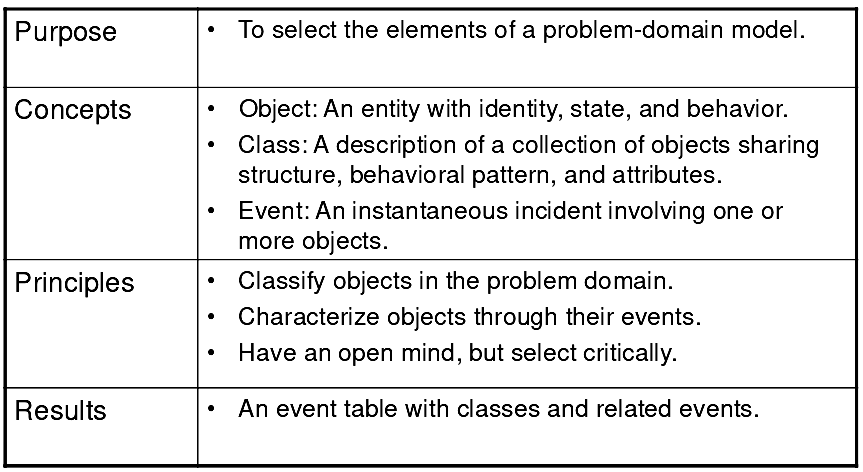
\includegraphics[width=0.75\textwidth]{figures/classessummary.png}
\end{figure}
\section{Challenges in this activity}
\begin{itemize}
    \item Classifying classes and events is mentally challenging %lol, wtf u mean Stage
    \begin{itemize}
        \item Difficult to find the right granularity
        \item Difficult to transcend the existing situation
    \end{itemize}
    \item Selecting the relevant classes and events is often difficult
    \begin{itemize}
        \item Use the criteria
        \item Be explicit about the reasoning for excluding
    \end{itemize}
    \item Functions are often described as events - but we usually do not want to register the application of a function
    \begin{itemize}
        \item Make a preliminary function list to remember them
    \end{itemize}
\end{itemize}

\section{Principles}
\subsection{Classify objects in the problem domain}
Make relevant abstractions and study reality. Focus on the problem domain and the different understandings that users have of it. Do not describe the application domain or the system itself.

\subsection{Characterise objects through their events}
Use events to understand the dynamics of the problem domain. It is the events that define the dynamic nature of objects and their mutual interplay.

\subsection{Have an open mind, but select critically}
Be open-minded and consider many candidates for classes and events. On the other hand, be critical and thorough in evaluating whether each class or event candidate is necessary in relation to the system definition.

\section{Exercises for lecture two}
\begin{itemize}
    \item Find candidates for classes
    \item Find candidates for events
    \item Select the relevant classes and events
    \item Be precise in the argumentation about which classes and events that should be included - \textit{use the criteria}
    \item Combine classes and events in an event table - \textit{which classes are involved in which events}
\end{itemize}
\subsection{Quiz}
12 minutes duration. 90\% correct answers.

\subsection{Exercise 3.6.16}
Classes:
\begin{itemize}
    \item Elevator
    \item Floor
    \item Button
    \item Passenger
    \item Request
    \item Sensors
    \item Door
    \item Call button
\end{itemize}

Events:
\begin{itemize}
    \item Door opened
    \item Door closed
    \item Button pressed
    \item Arrived at floor
    \item Floor left
    \item Elevator called
    \item Floor requested
    \item Elevator malfunctioned
    \item Light turned on
    \item Light turned off
    \item Turned on
    \item Turned off
\end{itemize}

\subsubsection{Event table}

\begin{table}[h]
\centering
\begin{tabular}{|l|l|l|l|l|l|}
\hline
 & Elevator & Floor & Button & Request & Sensor \\ \hline
Door opened & x & x &  &  & x \\ \hline
Door closed & x & x &  &  & x \\ \hline
Arrived at floor & x & x &  &  & x \\ \hline
Floor departed & x & x &  &  & x \\ \hline
Floor requested &  & x & x & x &  \\ \hline
Request fulfilled &  & x &  &  & \\ \hline
Elevator malfunctioned & x &  &  &  & x \\ \hline
Light turn on &  &  & x & x &  \\ \hline
Light turn off &  &  & x & x &  \\ \hline
Turned on & x &  & x & x &  \\ \hline
Turned off & x &  & x & x &  \\ \hline
\end{tabular}
\end{table}